\chapter{A finite element method for the Landau-Lifshitz-Gilbert Equation}
\label{sec:galerk-meth-llg}

In this chapter we introduce first give a general introduction to the finite element method.
We then apply the finite element method (with the Newton-Raphson method for linearisation) to the Landau-Lifshitz-Gilbert equation with exchange and a simple magnetostatic field approximation.

\section{Introduction to the finite element method}
\label{sec:intr-finite-ele-diff}

As discussed in \cref{sec:sd-finite-elem-meth} the finite element method (FEM) is a discretisation method which converts a differential equation into a system of algebraic equations.
It allows for more complex geometries than the finite difference method, at the cost of increased complexity.

A simple problem is used to illustrate these methods: solving the Poisson
equation in one spatial dimension.
This is relevant to 
Find\footnote{A function $g\in C^{k}(0,1)$ if $g$ and it's first $k$ derivatives are continuous on $(0,1)$.} $y(x)\in C^{2}(0,1)$ such that
\begin{equation}
  -y''=f\qquad\text{on }(0,1)
  \label{eq:poisson1}
\end{equation}
\begin{equation*}
  y(0)=y_{a},\quad y(1)=y_{b},\quad f=f(x)\in C(0,1).
\end{equation*}


\subsection{Definitions}
\label{sec:fem-definitions}

The function space $L^{2}$ is the set of all functions $f(x)$ such that $\int_{-\infty}^{\infty}\abs{f(x)}^{2} \d x$ is finite.
The span of a set of functions is the set of all possible linear combinations of the functions. 
If a set of functions $\set{\phi_i}$ is such that $V=\text{span}(\phi_i)$ then we say that $\set{\phi_i}$ spans $V$ and $\set{\phi_i}$ is a basis for the function space $V$.
If $V$ has a basis consisting of a finite number of functions then we say that $V$ is finite dimensional, otherwise $V$ is infinite dimensional.
In a FEM we are interested in approximating an infinite dimensional space (the space of solutions) by a finite dimensional space (the space of approximations).

The $n$-th Sobelov space is the space of all functions such that they and their $n$-th derivatives (in all dimensions) are in $L^2$. For example
\begin{equation}
  \label{eq:H1}
  \sob^1(\magd) = \set{ y \st y, \pd{y}{x_i} \in L^2(\magd) \; \forall x_i }
\end{equation}

\subsection{A weak formulation}
\label{Derivation-of-weighted-residuals}

The method of weighted residuals is a way to convert a differential equation
into an integral form that can be modelled computationally. As such it is the
first step in a variety of modelling methods including the finite element method
and the spectral method.

For simplicity we start, as before, with the one-dimensional Poisson equation
\cref{eq:poisson1}, with homogeneous Dirichlet boundary conditions
(\ie $y_{a}=y_{b}=0$).

The formulation used in \cref{eq:poisson1} (called a strong formulation) is too restrictive for our purposes.
It disallows some useful approximating functions, and in higher dimensional cases restricts the geometries that can be modelled \cite{HowardElmanDavidSilvester2006}. 
However for well behaved functions the following weak formulation is equivalent: find $y\in V_{s}$ such that
\begin{equation}
  -\int_{0}^{1}y''v\, dx=\int_{0}^{1}fv\, dx \qquad \forall v\in V_{T}.
  \label{eq:26}
\end{equation}

Here $V_{T}$ is some appropriate space of test functions. The test
functions must satisfy $V_{T}\subseteq \sob^0(0,1)$, in order to ensure that the integrals in \cref{eq:26} are well defined. 
Thus
\begin{equation}
  \label{eq:28}
  V_{T}=\set{v : [0,1] \rightarrow \real \st v \in \sob^0(0,1)}.
\end{equation}

The space $V_{s}$ is the solution space
\begin{equation}
  V_{s}=\set{ y : [0,1] \rightarrow \mathbb{R} \st y \in \sob^2(0,1),\, y(0) = y_{a},\, y(1) = y_{b}},
\end{equation}
\ie the space of functions that are sufficiently smooth for the integrals to be finite and that satisfy the boundary conditions.

To see that the weak form is equivalent to \cref{eq:poisson1} consider the case when $f(x) - y''(x)$ is non-zero at a point $x \in [0,1]$. 
Since \cref{eq:26} must hold for all functions we can choose a function which is non-zero at $x$ and hence the equality in \cref{eq:26} fails.
So $f(x) - y''(x) = 0$ must hold at all points inside the domain.
We call this the method of weighted residuals because we use an integral of the residual weighted by a test function to approximate the true equation \cite[210, 214]{Zeinkiewicz1967}.

The smoothness restrictions on our weak form approximation can be further reduced using integration by parts
\begin{equation}
  \intui{qp'} = \Big[ pq \Big]_{0}^{1} - \intui{p q'},
\end{equation}
applied to the left hand side of \cref{eq:26}.
Let $p=y'$ and $q=v$, then
\begin{equation}
  -\intui{ y''v } = -\Big[ y'v \Big]_{0}^{1} + \intui{ y'v' }.
  \label{eq:29}
\end{equation}

??ds mention Neumann

We now introduce a second constraint to the test functions: $v=0$
at the boundaries (\ie $v_a=v_b=0$), so the bracketed term in \cref{eq:29} is
zero and we are left with
\begin{equation}
  -\intui{ y''v } = \intui{ y'v' }.
\end{equation}

Hence our problem can be reduced to the following: find 
\begin{equation}
y\in V_{S}'=\set{y \st y \in \sob^1(0,1),\, y(0) = y_a, y(1) = y_b },
\end{equation}
such that
\begin{equation}
  \intui{ y'v' } = \intui{ fv } \qquad 
  \forall v \in V'_{T} = \set{v \st v \in \sob^1(0,1),\, v_a=v_b=0}.
  \label{eq:symmetric-weak-poisson}
\end{equation}

Note that this rearrangement has removed the second derivative in $y$, hence we only require $y \in \sob^1(0,1)$ instead of $y \in \sob^2(0,1)$.
This allows a wider range of shape functions to be used but comes at the expense of requiring more smoothness in the test functions.
Also note that if $y_a = y_b = 0$ then $V_{S}'=V_{T}'$, our test and solution spaces are identical.

\subsection{A Discretisation}

\Cref{eq:symmetric-weak-poisson} is still inapplicable as a computational method since the test (and solution) space is infinite dimensional (\ie the problem is still continuous).
So for the next step we approximate $V_{T}'$ by a finite dimensional function space $V_{T}^{h}\subset V_{T}'$ such that
\begin{equation}
  V_{T}^{h}=\text{span} \set{ \tbf_{\ndi} }_{n=1}^{N}
  = \set{v_h \st v_h = \sum_{n=0}^{N}\alpha_{\ndi} \tbf_{\ndi},\, \alpha_{\ndi} \in \real,\,
    v_a = v_b =0 },
  \label{eq:30}
\end{equation}
for some finite set of test basis functions $\tbf_{\ndi}$.
The distinction between the test functions and the test basis functions is often dropped.
Similarly, for $V_S$
\begin{equation}
  \label{eq:34}
  V_{S}^{h}=\text{span} \set{ \sbf_{l} }_{l=1}^{N_l}
  = \set{y_h \st y_h = \sum_{l=0}^{N_l}c_{l} \sbf_{l},\, c_{l} \in \real,\,
    y(0) = y_a,\, y(1) = y_b }.
\end{equation}
We call $\sbf_l$ the shape functions.
Different choices of $\tbf_{\ndi}$ and $\sbf_l$ lead to different methods, the choice corresponding to the finite element method will be discussed in \cref{sub:Actual-Finite-Elements}.
For now we continue with the conversion of the problem into a general discrete form.

We currently have the discrete weak formulation of \cref{eq:poisson1}: find $y_{h}\in V_{S}^{h}$ such that
\begin{equation}
  \intui{ y'_{h}v_{h}' } =\intui{ fv_{h} } \qquad\forall v_{h}\in V_{T}^{h}.
  \label{eq:discrete-weak-prob}
\end{equation}
Replacing $v_{h}$ from \cref{eq:discrete-weak-prob} by $\tbf_{\ndi}$ gives an equivalent set of conditions
\begin{equation}
  \intui{  y'_{h} \tbf_{\ndi}'  }  = \intui{ f\tbf_{\ndi} } \qquad n=0,\ldots,N,
  \label{eq:discrete_weak_test_fns_replaced}
\end{equation}

Since $y_{h}\in V_{S}^{h}$ we can also replace $y_{h}$ by a linear combination of the shape functions, \ie
\begin{equation}
  y_{h}=\sum_{l=0}^{N_l}c_{l}\sbf_{l},
  \label{eq:y-spans}
\end{equation}
where $c_l \in \real$ are (unknown) coefficients.

Substituting \cref{eq:y-spans} into \cref{eq:discrete_weak_test_fns_replaced} gives
\begin{equation}
  \sum_{l=0}^{N_l}c_{l}\intui{ \sbf_{l}'\tbf'_{\ndi} } =\intui{ f\tbf_{\ndi} } 
  \qquad n=0,\ldots,N.
  \label{eq:31}
\end{equation}

The functions $f$, $\tbf$ and $\sbf$ are known and so the integrals in \cref{eq:31} are just numbers (which must be calculated at some point, see \cref{sec:numer-eval-integrals}).
Hence we introduce a matrix $\Am$ and a vector $\mathbf{b}$ containing these numbers:
\begin{equation}
  \intui{ \sbf_{l}'\tbf'_{\ndi} } =\Am_{l\ndi},\qquad\intui{ f\tbf_{\ndi} } =b_{j},\label{eq:Aij_bj}
\end{equation}
and the problem is reduced to a system of linear equations
\begin{equation}
  A\mathbf{c} = \mathbf{b}.
  \label{eq:final_galerkin}
\end{equation}
This can be solved to find the vector of unknown coefficients $\mathbf{c}$ which can be substituted into \cref{eq:y-spans} to give an approximation for $y$.


\subsection{Finite Elements in One Dimension}
\label{sub:Actual-Finite-Elements}

To create a useable implementation of the methodology derived in \cref{Derivation-of-weighted-residuals} we must first define basis functions for the spaces $V_{T}^{h}$ and $V_S^h$.
For simplicity we choose the two types of basis functions to be the same: $\sbf_l = \tbf_l$.
This choice defines the Galerkin method (and results in a symmetric matrix $\Am$, if the original equation has the corresponding symmetry) \cite[215]{Zeinkiewicz1967}.

??ds think I need to mention piecewiseness and zero outside element, finite support = sparse

The overall aim is to approximate an arbitrary function at a finite set of points called the ``nodes'', $x_\ndi$, by a linear combination of a finite set of easy-to-work-with functions, $\tbf_\ndi$.
There are a variety of useful choices for $\tbf_\ndi$ but we will focus on a carefully constructed set of polynomials: the Lagrange interpolation basis functions, defined as
\begin{equation}
  L_\ndi(x)=\prod_{k\neq i}\Bigg(\dfrac{x-x_{k}}{x_\ndi-x_{k}}\Bigg).
\end{equation}
This definition results in the following useful properties of $L_{\ndi}(x)$
\begin{equation}
  \label{eq:35}
  L_{\ndi}(x_{\ndi}) =
  \begin{cases}
    1 & k = \ndi, \\
    0 & k \neq \ndi,
  \end{cases}
\end{equation}
since at each $x_{\ndi}$ with $k \neq \ndi$ one of the numerators is zero and at
$x = x_{\ndi}$ all of the numerators are equal to their corresponding denominator.

Polynomials are chosen because they are easy to manipulate computationally, for example differentiation and integration are simple even in higher dimensions.
Also note that an arbitrary level of accuracy can be achieved when approximating the a smooth function by piecewise polynomials, provided that the polynomials are only non-zero on a sufficiently small area (\ie after sufficient mesh refinement).

We now consider the simple case where we approximate the function at two points $x_{0}$ and $x_{1}$ (linear interpolation).
Then the Lagrange basis functions are simply
\begin{equation}
  L_{0}=\dfrac{x-x_{1}}{x_{0}-x_{1}},\qquad
  L_{1}=\dfrac{x-x_{0}}{x_{1}-x_{0}}.
  \label{eq:simple_lagrange}
\end{equation}
The interpolation of a function on the interval $[x_{0},x_{1}]$ is then given by
\begin{equation}
  y_{h}(x)=y(x_{0})L_{0}(x)+y(x_{1})L_{1}(x).
\end{equation}
It is advantageous to work with such low order polynomials even for very complex models because evaluation of integrals and interpolated values is simple and cheap to compute.
We can achieve this by splitting the domain into a set of $N$ \emph{elements} $e_{0},e_{1},\ldots,e_{N-1}$, each with a node at either end. % which can be of varying size (in contrast to the basic finite difference method where the nodes had to be equally spaced)
We then create a \emph{local} numbering scheme for the nodes and functions in each element and a \emph{global} numbering scheme to keep track of the same nodes and functions over the entire domain.

In one dimension the boundary of each element consists of two points, one at each end.
In the local scheme it is natural to label these points by the element number $e$ and a local node number, \ie $x_{0}^{(e)}$ and $x_{1}^{(e)}$.
In the global scheme each node is labelled by a unique node number, \ie $x_{\ndi}$ for $\ndi=0,\ldots,N$.
The concept is best illustrated by a diagram, see \cref{fig:local-global-numbering}.

\begin{figure}
  \center
  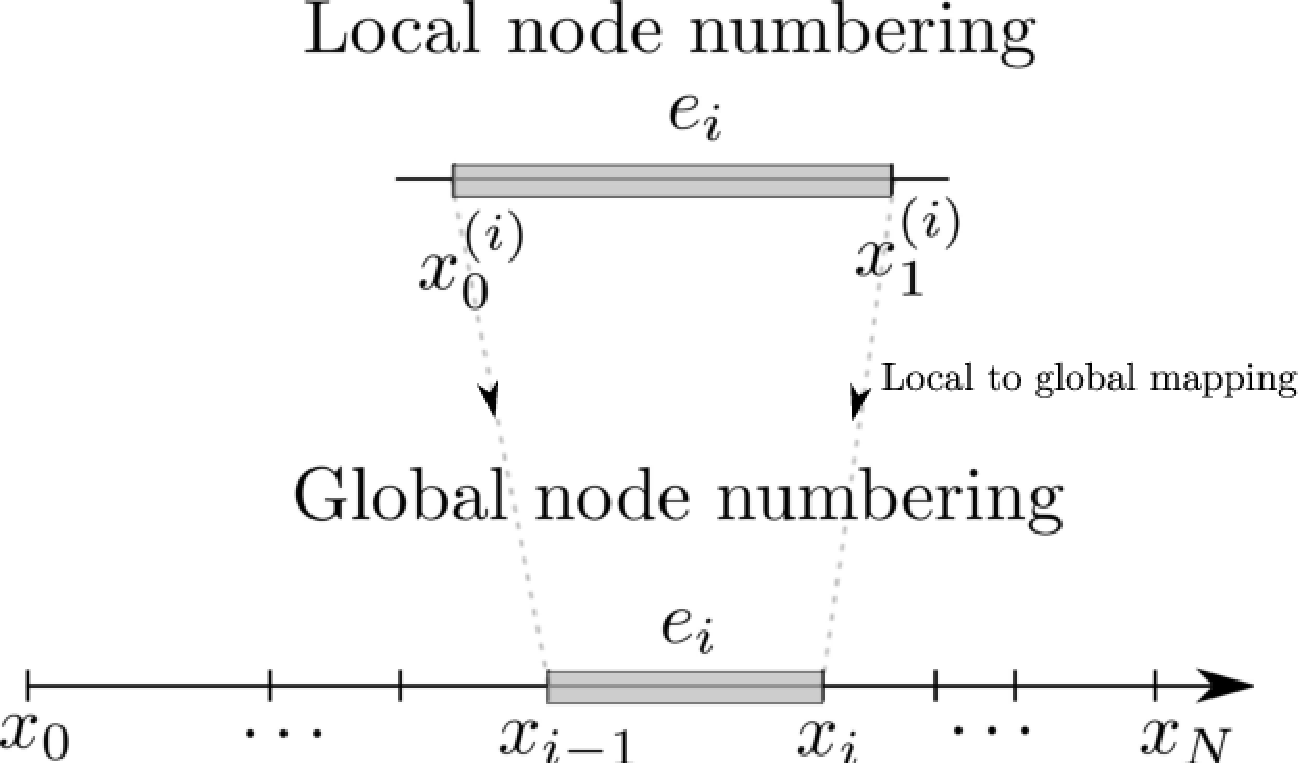
\includegraphics[width=0.8\textwidth]{./images/local_global_numbering}
  \caption{The local and global numbering schemes for nodes in a one-dimensional
    finite element model.}
  \label{fig:local-global-numbering}
\end{figure}

The process of assigning a global node number to each local node is known as the local to global mapping.
Good book keeping of the mapping is essential, especially in higher dimensions when this it becomes much more complex.

We define the local basis functions in element $e$ as
\begin{equation}
  L_{0}^{(e)}(x)=\dfrac{x-x_{1}^{(e)}}{x_{0}^{(e)}-x_{1}^{(e)}},\qquad
  L_{1}^{(e)}(x)=\dfrac{x-x_{0}^{(e)}}{x_{1}^{(e)}-x_{0}^{(e)}}
  \qquad\text{for }x\in e=[x_{0}^{(e)},x_{1}^{(e)}].
  \label{eq:32}
\end{equation}
Except for the test functions when $\ndi$ is a boundary node.
In this case we define $L_\ndi^{(e)} = 0$.
The $\ndi$th global basis function is then defined as:
\begin{equation}
  \label{eq:33}
  L_\ndi(x) =
  \begin{cases}
    L_\ndi^{(e)}(x) & \text{if node $\ndi$ is in element $e$,} \\
    0 & \text{otherwise.}
  \end{cases}
\end{equation}

\begin{figure}
  \center
  % ??ds numbering: change e_i to element e, e_{i+1} to e+1, x_i to x_\ndi, x^(i) to x^(e) L_i to L_\ndi
  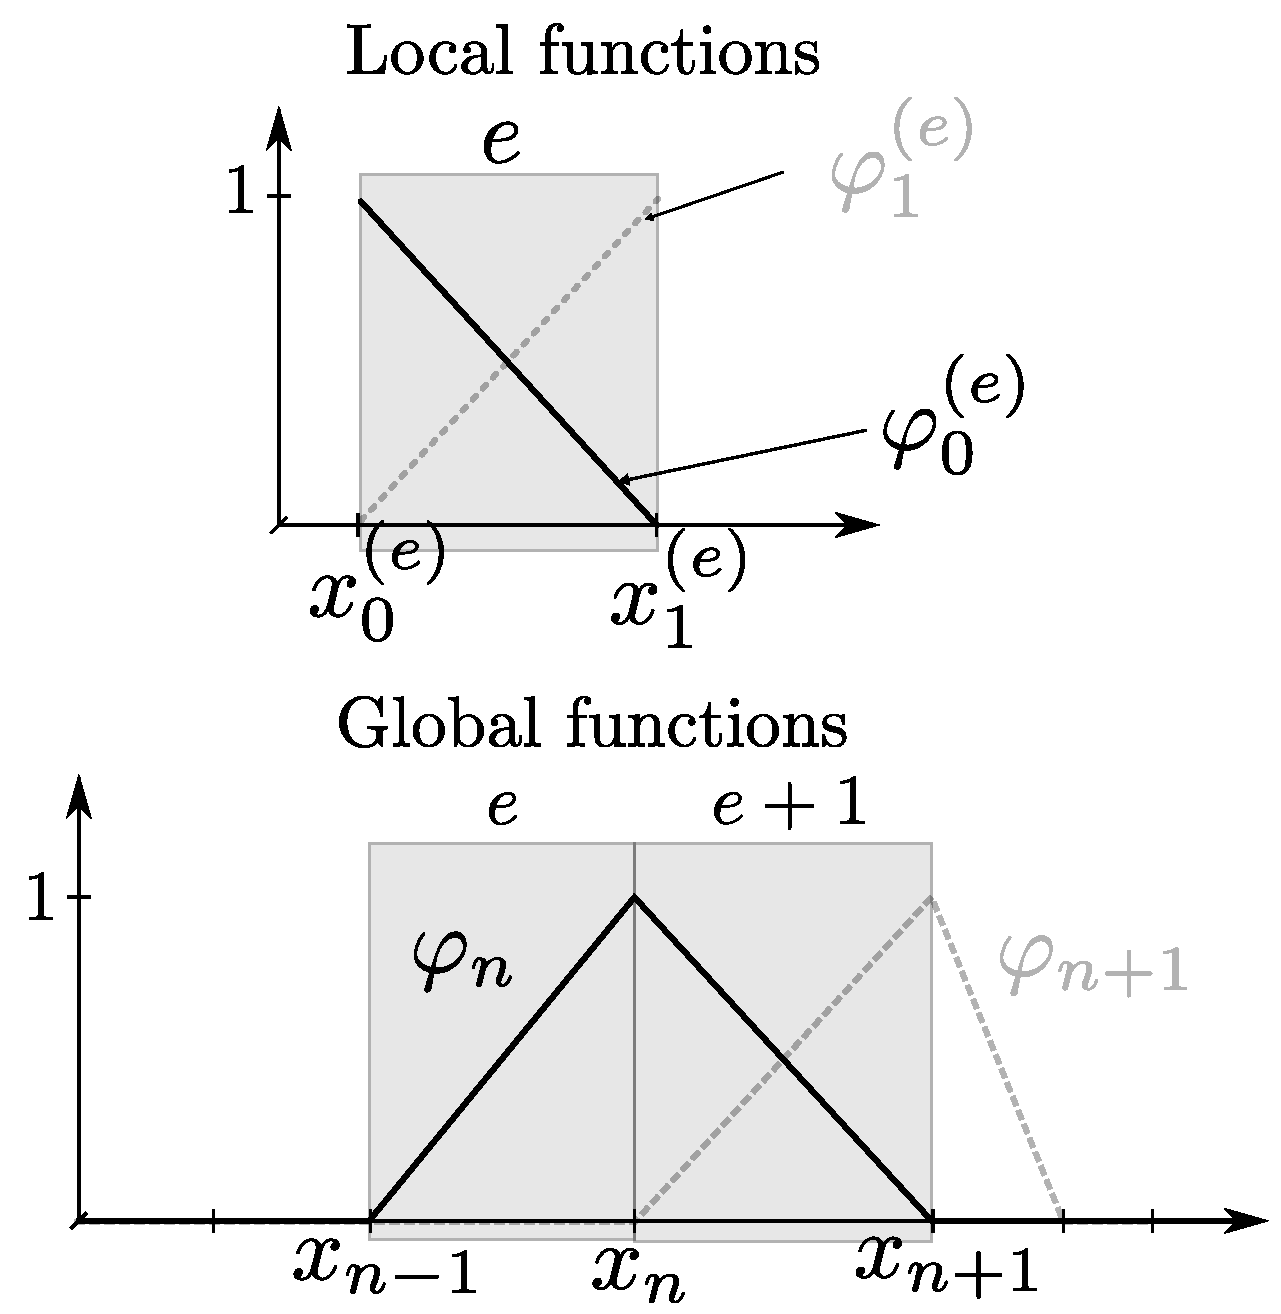
\includegraphics[width=0.8\textwidth]{./images/local_global_functions}
  \caption{The linear Lagrange basis functions and numbering schemes for a one-dimensional
    finite element model.\label{fig:local_global_functions}}
\end{figure}

The global basis functions for are clearly integrable (\ie in $L^2[0,1]$) since they are just a combination of local basis functions and they satisfy the boundary conditions by definition.
So the global basis functions are members of $V_T^h$ and $V_S^h$.

To calculate the matrix $\Am$ and the vector $\mathbf{b}$ from equation \cref{eq:Aij_bj} needed for \cref{eq:final_galerkin} we first calculate the local contributions from each element: $\Am^{(e)}$ and $\mathbf{b}^{(e)}$.
Then the local-to-global mapping tells us which local nodes map to a given global node and so the global matrix $\Am$ and vector $\mathbf{b}$ can be assembled by summing the appropriate local contributions.

For our one-dimensional Poisson case the calculation of $\Am^{(e)}$ is quite
simple, substituting the two local basis functions \cref{eq:32} into
\cref{eq:Aij_bj} and using $h=x_{1}^{(e)}-x_{0}^{(e)}$ we are left with
\begin{equation}
  \Am^{(e)} = \dfrac{1}{h}
  \left[
    \begin{array}{cc}
      1 & -1 \\ -1 & 1
    \end{array}
  \right],
\end{equation}
where $h$ is the element size, $h = x_{1}^{(e)}-x_{0}^{(e)}$ (note that $h$ can vary between elements).
Similarly for $\mathbf{b}^{{e}}$ we obtain
\begin{equation}
  \mathbf{b}^{(e)}=\dfrac{1}{h}\left[
    \begin{array}{c}
      -\int_{x_{0}^{(e)}}^{x_{1}^{(e)}}(x-x_{1}^{(e)})\, f(x)\, dx\\
      \int_{x_{0}^{(e)}}^{x_{1}^{(e)}}(x-x_{0}^{(e)})\, f(x)\, dx
    \end{array}\right],
\end{equation}
which we must compute numerically since the entries depend on $f(x)$ which is not fixed.



\subsection{Numerical evaluation of integrals}
\label{sec:numer-eval-integrals}

In the above example the integrals for $\Am$ were fixed and so could be calculated analytically.
This is not the case in general (\eg the vector $\bv$, or the matrix for non-linear problems), so we need some method to computational evaluate the integrals.
The most flexible way to evaluate integrals is to do it purely numerically using a quadrature scheme.
A quadrature scheme is an approximation to an integral of the form
\begin{equation}
  \begin{aligned}
    \intdx{f(\xv)} &\approx  \sum_i w_i f(\xv_i),
  \end{aligned}
\end{equation}
where the selection of the ``knots'' $\xv_i$ and the weights $w_i$ depend on the scheme.

There exist many different quadrature schemes suited for different applications.
However because we only ever need to evaluate integrals of polynomial functions a single simple and extremely accurate class of quadrature is sufficient: Gaussian quadrature \cite[492]{Kincaid2002}.
Gaussian quadrature is the quadrature scheme derived by choosing the knots such that when $n$ knots are used it is able to exactly evaluate integrals of polynomials up to order $2n + 1$ (this is the highest possible order).

In higher dimensions the integration is not quite so simple.
Quadrature schemes only apply over specificly shaped elements (or at least must be non-trivially modified for other geometries).
To get around this issue we use a coordinate transformation to a reference element \cite[29]{HowardElmanDavidSilvester2006}.
So \eg any four sided element is mapped to a square element $[-1, 1] \times [-1, 1]$, and standard quadrature schemes can be used.
The final difficulty is to calculate the Jacobian of the transformation: if the ``local'' position variable is $\sv$ then the Jacobian is
\begin{equation}
  J = \abs{ \pd{\sv}{\xv}} = \frac{1}{\abs{\pd{\xv}{\sv}}},
\end{equation}
where the elements of the Jacobian matrix $\pd{\xv}{\sv}$ can be calculated by interpolating $x$ using the local shape functions and differentiating.

So the final integration scheme is
\begin{equation}
  \begin{aligned}
    \intdx[\magd_e]{f(\xv)} &= \intds[\magd_e]{f_s(\sv) J_e(\sv)}, \\
    &\approx  \sum_{i=0}^N w_i f_s(\sv_i) J_e(\sv_i).
  \end{aligned}
\end{equation}
where the definition of $f_s(\sv)$ is
\begin{equation}
  f_s(\sv) = f\bigb{\sum_j  \xv_j \sbf_j(\sv)}.
\end{equation}

??ds use local coords in diagrams?

Gaussian quadratures for square and cube elements can be trivially constructed from the one dimensional quadrature using a tensor product formula.
Similar ``full integration'' quadratures for triangular and tetrahedral elements exist \eg \cite{oomph-lib-integral.cc}.




\section{Application to spatial discretisation of the LLG}
\label{sec:llg-initial-equations}

We now apply the methodology discussed in \cref{sec:intr-finite-ele-diff} to the Landau-Lifshitz-Gilbert equation.
We start with the Gilbert form of the LLG \cref{eq:Gilbert} with the various effective fields and the potential method for calculating the magnetostatic field \cref{eq:Hms}.
We use the Gilbert form of the Landau-Lifshitz-Gilbert equation even though it is less immediately intuitive because it greatly reduces the complexity of all derivatations--the Landau-Lifshitz form contains a double cross product term.
A side effect of this choice is that explict timestepping schemes cannot be used since the time dependence of the fundamental equation is defined implicitly.

\subsection{Initial equations}

After non-dimensionalisation (see \cref{sec:land-lifsh-gilb-normalisation}) the Landau-Lifshitz-Gilbert equation with effective fields is given by
\begin{equation}
  \begin{aligned}
    \dmdt &= - \mv \times \hv + \alpha \mv \times \dmdt, \\
    \hv &= \happ - \nabla \phim + \lap \mv + \kone (\mv \cdot \ev) \ev, \\
    \lap \phim &= \div \mv.
    \label{eqn:ndllg-starting}
  \end{aligned}
\end{equation}

For now we consider the magnetostatic potential only within the magnetic domain, $\magd$, with Neumann or Dirichlet boundary conditions on the boundary, $\boundd$. 
Details of the extension to include the effects of the external region using the FEM/BEM method are given in \cref{sec:hybr-finit-elem}, both Dirichlet and Neumann cases will be required.
We define $\boundd_D$ and $\boundd_\Neu$ respectively to represent the region of the boundary domain where a Dirichlet condition or Neumann is imposed on the potential.
So on $\boundd_\Neu$ $\nabla \phim(\xv) \cdot \nv = g_\Neu(\xv)$ and on $\boundd_D$ $\phim(\xv) = g_D(\xv)$.
We also define the following function spaces for convenience
\begin{equation}
\begin{aligned}
  \label{eq:037}
  \Dfs & = \set{ v \st v(\xv) = g_D(\xv) \; \forall \xv \in \boundd_D }, \\
  \Dfs_0 &= \set{ v \st v(\xv) = 0 \; \forall \xv \in \boundd_D }.
\end{aligned}
\end{equation}

Recall from \cref{sec:magn-bound-cond} that the boundary condition on the magnetisation is
\begin{equation}
  \label{eq:m-bc}
  \mv \times \dmdn = \zerov,
\end{equation}
It turns out that this Neumann-like condition is exactly what is needed in the derivation of the residuals.
No special function space is needed for the solutions and test functions of $\mv$ since only Neumann conditions are used.


\subsection{Conversion to Weak Form Residuals}

We now convert the above equations into their residual weak forms as described in \cref{Derivation-of-weighted-residuals}.
In the following we will need the identity\footnote{This can be easily derived by applying the product rule to $\nabla \cdot (v \nabla \phim)$.}
\begin{equation}
  (\lap \phim) \test = \nabla \cdot (v \nabla \phim) - \nabla \phim \cdot \nabla v.
  \label{eq:20}
\end{equation}
We will also make use of the divergence theorem
\begin{equation}
  \intd{\div \fv} = \intb{\fv \cdot \nv}.
  \label{eq:div-thm}
\end{equation}

The residual equation for the magnetostatic potential becomes
\begin{gather}
  \rphi(\phim) = \intd{ (\lap \phim) \test }
  - \intd{ (\nabla \cdot \mv) \test}, \label{eqn:phires1}
\end{gather}
where $\phim \in \sob^2(\magd) \cap \Dfs$, $\mv$ is some sufficiently smooth given function.
Recall that the  residual must be zero $\forall \test \in \sob^0(\magd) \cap \Dfs_0$.

The use of \cref{eqn:phires1} for calculating $\rphi$ would require the existence of second order derivatives.
We prefer to reduce the order of these derivatives as discussed in \cref{Derivation-of-weighted-residuals} to relieve the smoothness requirements on our solution.
As before we do this by ``transfering'' the derivatives onto the test functions \cite{HowardElmanDavidSilvester2006}.

Using identity \cref{eq:20} and the divergence theorem \cref{eq:div-thm} gives
\begin{equation}
  \begin{aligned}
    \intd{ (\lap \phim) \test} &=  \intd{\nabla \cdot (\test \nabla \phim)}
           - \intd{\nabla \phim \cdot \nabla \test},\\
    &= \intb{\test (\nabla \phim \cdot \nv)} 
    - \intd{ \nabla \phim \cdot \nabla \test}.
    \label{eqn:identitygauss}
  \end{aligned} 
\end{equation}

We now substitute \cref{eqn:identitygauss} into \cref{eqn:phires1} to find
\begin{equation}
  \rphi(\phim) = \intb{ \test (\nabla \phim \cdot \nv) }
  - \intd{ \nabla \test \cdot \nabla \phim }
  - \intd{ (\nabla \cdot \mv) \test },
\end{equation}
This contains only first order derivatives so the solution space for $\phim$ is relaxed to $\sob^1(\magd) \cap \Dfs$. 
However all first partial derivatives of the test functions are now required to be integrable, \ie $v \in \sob^1(\magd)$ instead of $v \in \sob^0(\magd)$.

Note that the boundary integral is always zero on the Dirichlet region of the boundary by our definition of the test functions. 
Hence the boundary integral is only non-zero over $\boundd_{\Neu}$ where we know $(\nabla \phim \cdot \nv) = g_{\Neu}$.
So the final residual is
\begin{equation}
  \rphi(\phim) = \int_{\boundd_\Neu} \test g_\Neu \d \boundd
  - \intd{ \nabla \test \cdot \nabla \phim}
  - \intd{ (\nabla \cdot \mv) \test}.
  \label{res:contphi}
\end{equation}


For the Landau-Lifshitz-Gilbert equation, \cref{eqn:ndllg-starting}, we have a set of three residuals per test function. 
For now we sidestep the details of time discretisation by assuming $\dmdt$ to be just another function of $\xv$.
\begin{equation}
  \rllgv(\mv, \test) = \int_\magd \Big( \dmdt
  + (\mv \times \hca) + (\mv \times \happ) \\
  - (\mv \times \nabla \phi) + (\mv \times \lap \mv)
  - \dampc \left( \mv \times \dmdt \right)
  \Big) \test \d\magd
  . \label{res:contllg}
\end{equation}
Similarly to the previous examples the aim is to find $\mv \in \sob^2(\magd)$ such that $\rllgv(\mv, \test) = 0$ $\forall \test \in \sob^0(\magd)$.

Note that in \cref{res:contllg} the residual is a vector, it is equivalent to write
\begin{equation}
  \rllg(\mv, \testv) = \int_\magd \Big( \ldots  \Big) \cdot \testv \d\magd,
\end{equation}
where $\testv \in (\sob^0(\magd))^3$.
To see that $\rllg(\mv, \testv) = 0\; \forall \testv \in (\sob^0(\magd))^3$ implies $\rllg(\mv, \test) = 0 \; \forall \test \in \sob^0(\magd)$ consider three vector test functions: $(\test, 0, 0)$, $(0, \test, 0)$ and $(0, 0, \test)$.
Clearly $\rllg(\mv, (\test, 0, 0)) = \rllg(\mv, \testv)[0]$, and similarly for the other two cases.
To see the inverse: note that if $\rllg(\mv, \test) = 0\; \forall \test \in \sob^0(\magd)$ then each term of every dot product in $\rllg(\mv, \testv) \; \forall \testv \in (\sob^0(\magd))^3$ is zero, and so each total residual is zero.
The use of vector test functions makes certain manipulations simpler so, for the rest of this section, we will work with a vector test function.

We again wish to reduce the order of the required derivatives, this time on $\mv$ in the term
\begin{equation}
  I = \intd{ (\mv \times \lap \mv) \cdot \testv }.
  \label{eq:46}
\end{equation}
First we reorder the terms to give
\begin{equation}
  \begin{aligned}
    I &= \intd{\lap \mv \cdot (\testv \times \mv)}, \\
      &= \intd{\lap \mv \cdot \bv}, \\
      &= \sum_{i=0}^2 \intd{ b_i (\lap m_i)},
  \end{aligned}
\end{equation}
where $\bv = (\testv \times \mv)$.
Note that this is very similar to \cref{eqn:phires1}, and so we can apply the same operations as were used to obtain reduced derivatives in the Poisson case. 
Doing so we obtain
\begin{equation}
  I = \sum_{i=0}^2 \intb{b_i (\grad m_i \cdot \nv)} - \intd{\grad b_i \cdot \grad m_i}.
\end{equation}

It turns out that the first term is exactly the weak form of the boundary condition from \cref{eq:m-bc}.
\begin{equation}
  \begin{aligned}
    \sum_{i=0}^2 \intb{b_i (\grad m_i \cdot \nv)} 
    &= \intb{\bv \cdot \pd{\mv}{\nv}}, \\
    &=  \intb{(\testv \times \mv) \cdot \pd{\mv}{\nv}}, \\
    &=  \intb{(\mv \times \pd{\mv}{\nv}) \cdot \testv} = 0 .
  \end{aligned}
\end{equation}

Next we need an expression for $\grad b_i$.
To avoid switching to tensor notation it is helpful to define, for any vector $\av$: $\grad \av = (\grad a_0, \grad a_1, \grad a_2)$.
Then using the product rule we have
\begin{equation}
  \begin{aligned}
    \grad \bv &= \grad \bigb{\testv \times \mv}, \\
    & = (\grad \testv) \times \mv + \testv \times (\grad \mv).
  \end{aligned}
\end{equation}
Hence
\begin{equation}
  I = - \intd{\grad \mv : \bigb{\grad \testv \times \mv}} 
      - \intd{\grad \mv : \bigb{\testv \times \grad \mv}},
      \label{eq:72}
\end{equation}
where ``$:$'' is the componentwise scalar product, \eg $\grad \av : \grad \cv = \grad a_0 \cdot \grad b_0 + \grad a_1 \cdot \grad b_1 + \grad a_2 \cdot \grad b_2$.

Note that the $:$ operator obeys the usual triple product identity
\begin{equation}
  \av : (\av \times \bv) = \zerov,
  \label{triple:-identity}
\end{equation}
and it's permutations because
\begin{equation}
  \begin{aligned} 
    \threevecnum{\av} : \bigb{\threevecnum{\av} \times \bv} &= \av_0 \cdot (\av_0 \times \bv) + \ldots, \\
    & = 0 + 0 + 0
  \end{aligned}
\end{equation}

Hence the second term of \cref{eq:72} is zero and after reordering some terms we are left with
\begin{equation}
  \label{eq:final-lap-residual}
  I = - \intd{\bigb{\mv \times \grad \mv} : \grad \testv}.
\end{equation}

So the final residual for the LLG equation, using a vector test function, is
\begin{equation}
  \begin{aligned}
    \label{eq:llg-res-final}
    \rllg(\mv, \testv) &= \int_\magd \dmdt\cdot \testv
    + (\mv \times \hca)\cdot \testv 
    + (\mv \times \happ)\cdot \testv 
    - (\mv \times \nabla \phi)\cdot \testv \\
    & - \bigb{\mv \times \grad \mv} : \grad \testv
    - \dampc \left( \mv \times \dmdt \right)\cdot \testv
    \d\magd.
  \end{aligned}
\end{equation}

The final problem statement is: 
\begin{equation}
  \eqpar{Find $\mv \in (\tsinf)^3$, $\phim \in \tsinf \cap \Dfs$ such that $\rllg(\mv, \testv) = 0$ for all $\testv \in (\tsinf)^3$ and $\rphi(\phim, \test) = 0$ for all $\test \in \tsinf \cap \Dfs_0$.}
\label{eq:inf-dim-problem}
\end{equation}




\subsection{Spatial Discretisation}
\label{sec:spat-discr-resi}

The next step is to choose a finite dimensional approximation, $\ts$, for the infinite dimensional test and solution function spaces, $\tsinf$, such that the residuals \cref{res:contphi,eq:llg-res-final} become discrete in space.
Just as in \cref{sub:Actual-Finite-Elements} we represent the finite dimensional spaces using a set of piecewise linear polynomials, $\tsbasis$, as basis functions.

The approxmiations to the unknown functions $\mv$ and $\phim$ are represented as a sum over the shape functions $\sk \in \tsbasis$ (or $\tsbasis \cap \Dfs$ for $\phim$ with Dirichlet conditions) as
\begin{equation}
  \begin{aligned}
    \mv &\approx \sum_{k = 0}^{N} \sk \, \mv_k, \\
    \phim &\approx \sum_{k = 0}^{N} \sk \, \phim_{k}.
    \label{eq:unknowns-basis}
  \end{aligned}
\end{equation}
Similarly the approximations to the test functions are represented as a sum over the test basis functions, $\tn \in \tsbasis$ (or $\tsbasis \cap \Dfs_0$ as applicable), as
\begin{equation}
  \label{eq:47}
  \test \approx \sum_{\ndi = 0}^{N} \tn \, a_\ndi.
\end{equation}
Note that in our method $\sbf_k \equiv \tbf_k$ except for Dirichlet boundary $\phim$ shape functions, but we continue to write them differently for generality.
In one dimension the $\sk$ and $\tn$ are as given in \cref{eq:simple_lagrange}.
The extension to higher dimensions is straightforward: see \eg \cite[25]{HowardElmanDavidSilvester2006}.

So substituting the basis representations, \cref{eq:unknowns-basis,eq:47} into the continuous residuals we obtain approximations for the residuals in terms of a finite number of nodal values.\footnote{We do not write this form out here as it is long, messy and does not illuminate anything.}
Next we replace the requirement that the residuals be zero for all test functions in the infinite dimensional set $\tsinf$ with the equivalent requirement for all functions in the finite set $\tsbasis$. 
This results in a finite number of conditions (the residuals) on a finite number of variables (the nodal values) and so the spatial discretisation is complete.

As described in \cref{sub:Actual-Finite-Elements} we also convert this ``global'' representation into a number of ``local'' representations--one on each element.

% Let $\magd_\eli$ represent the volume of element $e$, let $\boundd_\eli$ represent any part of the boundary of the element which is on $\boundd$ (nothing for most elements).
% Then the contribution of element $\eli$ to the residuals at node $\ndi$ is exactly as given in equations~\cref{res:tintro}-\cref{res:tllg} except that the integrations are performed over $\magd_\eli$ and $\boundd_\eli$ rather than $\magd$ and $\boundd$.
% Also note that the sums only need to consider values of $k$ such that node $k$ is in element $\eli$ and that residual contributions only need to be calculated for nodes $\ndi$ such that node $\ndi$ is in element $\eli$.


\section{Time Discretisation}
\label{sec:time-discretisation-resi}

In this section we discuss how to deal with the time derivative in the LLG residual \cref{eq:llg-res-final}.
As discussed in \cref{sec:numer-meth-micr}, we will apply standard time integration methods used for ODEs.
This application of independent spatial and time discretisations is known as semi-discretisation or the method of lines.

We cannot simply apply the time integration methods in the way they are written in \cref{sec:some-implicit-time-integrators} (and in most text books) because our LLG residual \cref{eq:llg-res-final} cannot be written in the required form $\pd{\yv}{t} = \fv(t, \yv)$ since it is an implicit function of the time derivative.\footnote{Actually we could have started with the LL form \cref{eq:LLG} where the derivative can be given explicitly, but as mentioned above this method is simpler.}
Instead we rearrange the time integration method to give discrete substitutions for the time derivative, $\yv$ values and $t$.

Let $\dtn$ be the size of the $n$th time step, let $x_n$ denote value of $x$ at the $n$-th time-step.\footnote{This notation has some potential to be confused with the nodal value notation of \cref{sec:spat-discr-resi}, hopefully the meaning will be clear from the context.}
The simplest case is the first order backwards difference method (BDF1), which is defined by the substitution
\begin{equation}
  \begin{aligned}
    \pd{\yv}{t} &\rightarrow \frac{\yv_{n+1} - \yv_n}{\dtn}, \\
    \yv &\rightarrow \yv_{n+1}, \\
    t &\rightarrow t_{n+1}.
    \label{eq:impl-bdf1}
  \end{aligned}
\end{equation}
This substitution can be obtained by simple algebraic rearrangements of \cref{eq:bdf1-definition}.
Similarly the second order backwards difference method (BDF2) can be found (with some more complex algebra) to be:
\begin{equation}
  \begin{aligned}
    \pd{\yv}{t} &\rightarrow \yv_{n+1}\bigb{\frac{1}{\dtn} + \frac{1}{\dtn + \dtx{n-1}}}
    - \yv_n \frac{\dtn + \dtx{n-1}}{\dtn\dtx{n-1}}
    + \yv_{n-1} \frac{\dtn}{(\dtn + \dtx{n-1})\dtx{n-1}}, \\
    \yv &\rightarrow \yv_{n+1}, \\
    t &\rightarrow t_{n+1}.
    \label{eq:impl-bdf2}
  \end{aligned}
\end{equation}

The implicit midpoint rule is defined by the substitutions
\begin{equation}
  \begin{aligned}
    \pd{\yv}{t} &\rightarrow \frac{\yv_{n+1} - \yv_n}{\dtn}, \\
    \yv &\rightarrow \frac{\yv_{n+1} + \yv_n}{2}, \\
    t &\rightarrow \frac{t_{n+1} + t_n}{2}.
    \label{eq:impl-imr}
  \end{aligned}
\end{equation}
Alternatively, as mentioned in \cref{sec:some-implicit-time-integrators}, we can define the implicit midpoint rule in terms a step of BDF1 with $\dtn^\bdfo = \dtn^\imr/2$ to obtain $\yv_{n+\half}$ followed by the algebraic update
\begin{equation}
  \begin{aligned}
    \label{eq:imr-bdf1}
    \yv_{n+1} &= 2\yv_{n+\half} - \yv_n.
  \end{aligned}
\end{equation}

The trapezoid rule (TR) is defined (recursively) by
\begin{equation}
  \begin{aligned}
    \pd{\yv}{t} &\rightarrow \evalatb{\pd{\yv}{t}}{n+1} 
    = \frac{2(\yv_{n+1} - \yv_n)}{\dtn} - \evalatb{\pd{\yv}{t}}{n}, \\
    \yv &\rightarrow \yv_{n+1}, \\
    t &\rightarrow t_{n+1}.
    \label{eq:impl-tr}
  \end{aligned}
\end{equation}

So by applying one of the substitutions \cref{eq:impl-bdf1}-\cref{eq:impl-tr} to the system of spatially discretised residuals we obtain a fully discrete problem.
The properties of these time discretisations are exactly as discussed in \cref{sec:time-discretisation}.




\section{The analytical Jacobian}
\label{sec:llg-jacobian-calculation}

To solve our fully discrete system by a Newton method we also need to know the Jacobian matrix of each residual differentiated with respect to the $(n+1)$th variable at the time step.
This can be handled by numerical differentiation (\eg by approximating each derivative using a finite difference method), but analytical Jacobians are typically faster to compute and give better convergence properties than numerical approximations.
Additionally for the solution of the linear systems it is often useful to know analytically the structure of the system being solved.

Note that the ``real'' implementation of the implicit midpoint rule \cref{eq:impl-imr} introduces a factor of $1/2$ in various places due to the substitution $ \yv \rightarrow \frac{\yv_{n+1} + \yv_n}{2}$, the derivations below do not include this ??ds yet?

For this section we must use the scalar test function form of the residuals (since that is the form used in our final implementation).

We first note that the effect of differentiation by a nodal value on the function $\phim$ is quite simple:
\begin{equation}
  \begin{aligned}
    &\pd{\phim}{\phim_l} = \pd{}{\phim_l} \bigs{ \sum_k \phim_k \sk } = \sbf_l, \\
    &\pd{\phim}{\mv_l} = \pd{}{\mv_l} \bigs{ \sum_k \phim_k \sk } = \zerov^T, \\
  \end{aligned}
\end{equation}
and similarly for the interpolated magnetisation, $\mv$:
\begin{equation}
  \begin{aligned}
    &\pd{\mv}{\mv_l} = \pd{}{\mv_l} \bigs{ \sum_k \mv_k \sk } = \sbf_l \text{I}_3, \\
    &\pd{\mv}{\phim_l} = \pd{}{\phim_l} \bigs{ \sum_k \mv_k \sk } = \zerov, \\
\end{aligned} 
\end{equation}

\subsection{Poisson Jacobian}
\label{sec:poisson-jacobian}

Starting from the Poisson residual, \cref{res:contphi}, and dropping terms that obviously contain no dependence on $\phim_k$ we get
\begin{equation}
  \begin{aligned}
    \label{eq:poisson-jacobian}
    \Am_{n,l} &= \pd{}{\phim_{l}} \sum_k \intd{ -(\nabla \tbf_n \cdot \nabla \sbf_k) \phim_{k}}, \\
    &= -\intd{\grad \tbf_n \cdot \grad \sbf_l}.
  \end{aligned}
\end{equation}
This block of the Jacobian is comparatively simple because the Poisson equation is linear. 
It corresponds to the well known discrete Laplacian operator \cite{HowardElmanDavidSilvester2006}.


\subsection{LLG Jacobian}
\label{sec:llg-jacobian}

Unfortunately in most of the Jacobian calculations we have multiple terms depending on $\mv$ joined together by a cross product.
The process of differentiating these terms can be made much easier by making use of the ``skew operator'' which represents a cross product as a small matrix-vector multiplication.
The skew operator is given by
\begin{equation}
  \skewm{\av} = \text{skew}(\av) =
  \begin{pmatrix}
    0 & -a_3 & a_2 \\
    a_3 & 0 & -a_1 \\
    -a_2 & a_1 & 0
  \end{pmatrix}.
  \label{eqn:skew}
\end{equation}

Written using this skew operator the LLG residual is
\begin{equation}
  \begin{aligned}
    \rllgv_n = \int_{\magd}
    & \dmdt \tbf_n + \skewm{\mv} \cdot \left( \happ + \hca - \nabla \phi - \dampc \dmdt
    \right) \tbf_n \\
    &- (\skewm{\mv} \grad \mv) : \grad \tbf_n)
    \d\magd.
  \end{aligned}
\end{equation} 

Some useful properties of this skew operator are:
\begin{itemize}
\item Skew-matrix-vector multiplication is the cross product
  \begin{equation}
    \skewm{\av} \cdot \bv
    = \begin{pmatrix}
      0 & -a_3 & a_2 \\
      a_3 & 0 & -a_1 \\
      -a_2 & a_1 & 0
    \end{pmatrix}
    \cdot \threevec{b_1}{b_2}{b_3}
    = \threevec{-a_3b_2 + a_2b_3}{a_3b_1 - a_1b_3}{-a_2b_1 + a_1b_2}
    = \av \times \bv.
  \end{equation}

\item The skew operator has no effect on derivatives and vice-versa
  \begin{equation}
    \pd{}{x} \skewm{\av} = \skewm{ \pd{\av}{x} }.
  \end{equation}

\item The skew operator is linear
  \begin{equation}
    \skewm{\av + c \bv} = \skewm{\av} + c \skewm{\bv}.
  \end{equation}

\item It is easy to represent the Jacobian of a cross-product using the skew operator.
  The derivative with respect to $a_1$ is: 
  \begin{equation}
    \pd{}{a_1} \skewm{\av} \cdot \bv = \begin{pmatrix}
      0 & 0 & 0 \\
      0 & 0 & -1 \\
      0 & 1 & 0
    \end{pmatrix}\bv = \threevec{0}{-b_3}{b_2}.
  \end{equation}
  Note that this is the first column of $-\skewm{\bv}$, it turns out that
  \begin{equation}
    \pd{}{\av} \skewm{\av} \cdot \bv = \begin{pmatrix}
      0 & b_3 & -b_2 \\
      -b_3 & 0 & b_1 \\
      b_2 & -b_1 & 0
    \end{pmatrix} = -\skewm{\bv}.
    \label{eq:61}
  \end{equation}
  This is the main reason for preferring to calculate the Jacobian using this notation.
\end{itemize}

Due to the linearity of the skew operator we can write the Jacobian of a cross product including an interpolated value as 
\begin{equation}
  \begin{aligned}
    \pd{}{\mv_l} \bigb{\skewm{\mv} \bv} &= \pd{}{\mv_l} \skewm{\intp{\mv}} \bv, \\
    &= \sum_k \sbf_k \pd{}{\mv_l} \bigb{\skewm{\mv_k} \bv},
  \end{aligned} 
\end{equation}
then using the fact that the entries of $\pd{\mv_{l}}{\mv_{k}}$ are zero for $l \neq k$ we get
\begin{equation}
  \pd{}{\mv_l} \bigb{\skewm{\mv} \bv}  = \sbf_l \pd{}{\mv_l} \bigb{\skewm{\mv_l} \cdot \bv}.
\end{equation}
Next by using \cref{eq:61} we obtain
\begin{equation}
  \pd{}{\mv_l} \bigb{\skewm{\mv} \bv} = - \sbf_l\skewm{\bv},
  \label{eq:diff-skew-interp}
\end{equation}
finally by combining \cref{eq:diff-skew-interp} with the product rule we obtain the identity
\begin{equation}
  \begin{aligned}
    \pd{}{\mv_l} \bigb{\skewm{\mv}\cdot \gv(\mv)} 
    &= \skewm{\mv}\cdot \pd{\gv(\mv)}{\mv_l} - \sbf_l \skewm{\gv(\mv)}.
    \label{eq:68}
  \end{aligned}
\end{equation}
This provides us with a simple representation for almost all of the terms in the LLG Jacobian.

% As a simple example of how this can be used we first examine the differentiation of the $\mv \times (\happ + \hms)$ term of the Landau-Lifshitz equation residual (note that these two fields are not directly dependent on $\mv$).
% \begin{equation}
%\begin{aligned}
%   \circled{c} &= \mv \times (\happ + \hms),\\
%               &= \skewm{\mv} \cdot (\happ + \hms).
% \end{aligned}
%\end{equation}
% Now it is easy to see that applying \cref{eq:68} with $\gv = \happ + \hms$ gives us the Jacobian contribution
% \begin{equation}
%\begin{aligned}
%   \pd{}{\mv_l} \circled{c} = - \sbf_l \skewm{\happ + \hms},
% \end{aligned}
%\end{equation}
% since $\pd{\gv(\mv)}{\mv_l} \equiv 0$.


Now we calculate the Jacobian itself. 
To simplify the calculations we write the Jacobian as the sum of the individual terms:
\begin{equation}
  \begin{aligned}
    \Fm_{n,l} &= \pd{\rllgv_n}{\mv_l} = A_{n,l} + B_{n,l} + C_{n,l} + D_{n,l}, \\
    A_{n,l} &= \pd{}{\mv_l} \intd{\dmdt \tbf_n}, \\
    B_{n,l} &= \pd{}{\mv_l} \intd{- \skewm{\mv} \cdot (\grad \mv \compdot \grad \tbf_n)}, \\
    C_{n,l} &= \pd{}{\mv_l} \intd{ \skewm{\mv} \cdot \hca  \tbf_n}, \\
    D_{n,l} &= \pd{}{\mv_l} \intd{  \skewm{\mv} \cdot \bigb{ \happ - \nabla \phi - \dampc \dmdt} \tbf_n}.
  \end{aligned}
\end{equation}

First we the contribution due to the lone time derivative on the LHS:
\begin{equation}
  \begin{aligned}
    A_{n,l} &= \pd{}{\mv_l} \intd{ \dmdt \tbf_n } \\
           &= \jts \Idm_3 \intd{ \sbf_l \tbf_n}.
  \end{aligned}
\end{equation}
This is a $3\times3$ block diagonal matrix where each block is a simple mass matrix multiplied by a constant depending on the time integration method.

Next we calculate the contribution from the damping, applied field and magnetostatic field.
If we write the damping term in the form of \cref{eq:68} we have $\gv(\mv) = \dmdt$, so
\begin{equation}
  \label{eq:69}
  \pd{\gv(\mv)}{\mv_l} = \pd{}{\mv_l} \left(\pd{\mv}{t} \right) = \jts \sbf_l \Idm_3,
\end{equation}
where $\jts$ is the constant that multiplies $\mv_{n+1}$ in the approximation of the time derivative, for example when using the implicit midpoint rule $\jts = 1/\dtn$.
Now using \cref{eq:68} with \cref{eq:69} we immediately obtain
\begin{equation}
  \begin{aligned} 
    D_{n,l} &= \pd{}{\mv_l} \intd{  \skewm{\mv} \cdot
      \left( \happ - \nabla \phi - \dampc \dmdt
      \right) \tbf_n}, \\
    &= \int_\magd \tbf_n \big( -\sbf_l\skewm{\happ} + \sbf_l\skewm{\nabla \phi} + \dampc\sbf_l \skewm{\dmdt} - \dampc\sbf_l \jts \skewm{\mv} \Idm_3
    \big) \d\magd, \\
    &= \intd{ \tbf_n \sbf_l \bigb{ \skewm{-\happ + \nabla \phi 
          + \dampc \dmdt - \dampc \jts \mv}}}. \\
  \end{aligned}
\end{equation}
This is a $3\times3$ skew-symmetric matrix where each element is something like a mass matrix element multiplied by a collection of field/magnetisation components.

Now the contribution due to magnetocrystalline anisotropy.
Writing the residual in the form of \cref{eq:68} we have 
\begin{equation}
  \gv(\mv) = \hca = \kone (\mv \cdot \ev) \ev,  
\end{equation}
and so 
\begin{equation}
  \begin{aligned}
    \pd{\gv(\mv)}{\mv_l} &= \pd{}{\mv_l} \bigb{ \kone (\mv \cdot \ev) \ev}, \\
    &= \kone \bigb{ \pd{}{m_{x,l}} (\mv \cdot \ev), 
      \pd{}{m_{x,l}} (\mv \cdot \ev),
      \pd{}{m_{x,l}} (\mv \cdot \ev) }  \tensorprod \ev, \\
    &= \kone \sbf_l \; \ev  \tensorprod \ev.
    \label{eq:70}
  \end{aligned}
\end{equation}
Then combining \cref{eq:68,eq:70} we obtain
\begin{equation}
  \begin{aligned} 
    C_{n,l} &= \pd{}{\mv_l} \intd{ \skewm{\mv} \cdot \hca  \tbf_n}, \\
    &= \intd{ -\tbf_n \sbf_l\skewm{\hca} 
       + \kone \tbf_n \sbf_l \skewm{\mv} \; (\ev  \tensorprod \ev) }.
  \end{aligned}
\end{equation}
This term is a full $3\times3$ matrix in general, but note that if $\ev$ is aligned with the axes (as is typical) then only one entry of $(\ev  \tensorprod \ev)$ is non-zero.

Finally we calculate the exchange contribution.
We first need an identity
\begin{equation}
  \begin{aligned}
    \pd{}{\mv_l} \left(\nabla \mv \compdot \nabla \tbf\right) 
    &= \pd{}{\mv_l} \threevecdup{\left( \sum_k \mv_k \grad \sbf_k \right) \cdot \grad \tbf}, \\
    &=  \sum_k \pd{\mv_k}{\mv_l} \threevecdup{\grad \sbf_k \cdot \grad \tbf}, \\
    &=  \Idm_3 \left(\nabla \sbf_l \cdot \nabla \tbf \right).
    \label{eq:71}
  \end{aligned}
\end{equation}
Then using \cref{eq:68,eq:71} we get
\begin{equation}
  \begin{aligned}
    B_{n,l} &=  \pd{}{\mv_l} \intd{- \skewm{\mv} \cdot (\grad \mv \compdot \grad \tbf_n)} ,\\
    &= \intd{ \sbf_l \skewm{\grad \mv \compdot \grad \tbf_n}
       - \skewm{\mv} \left( \nabla \sbf_l \cdot \nabla \tbf_n \right)}, \\
     &= \intd{\skewm{ \sbf_l \grad \mv \compdot \grad \tbf_n
       - \mv \left( \nabla \sbf_l \cdot \nabla \tbf_n \right)}},
   \end{aligned}
 \end{equation}
which is a skew-symmetric $3\times 3$ matrix with each element something like an element of a  discrete Laplacian (\ie two derivatives). 

When written in block form the total LLG Jacobian is
\begin{equation}
  \Fm =
  \begin{pmatrix}
    \jts \Mm    & -\Km_z       & \Km_y \\
    \Km_z         & \jts\Mm    & -\Km_x \\
    -\Km_y        & \Km_x        & \jts \Mm
  \end{pmatrix} + \Jmca,
\end{equation}
where $\Mm$ is the mass matrix
\begin{equation}
  \label{eq:mass-matrix}
  \Mm_{i,j} = \intd{\tbf_i \sbf_j};
\end{equation}
$\Km_i$ are the skew-symmetric contributions from $B$, $C$ and $D$; and
\begin{equation}
  \Jmca = \kone \skewm{\mv} \; (\ev  \tensorprod \ev).
\end{equation}

\subsection{LLG-magnetostatics coupling Jacobians}
\label{sec:llg-magn-coupl}

In this section we derive the Jacobian entries corresponding to $\Pm = \pd{\rllgv}{\phim}$ and $\Qm = \pd{\rphi}{\mv}$.

First $\Pm_{n,l}$, this is a $3 \times 1$ matrix because we are dealing with a vector of three residuals at once.
Obviously most of the terms in the llg residual are dropped when differentiated with respect to any $\phim_{l}$ so the calculation is quite simple
\begin{equation}
  \begin{aligned}
    \Pm_{n,l} &= \pd{\rllgv_n}{\phim_l} 
    = \pd{}{\phim_l} \intd{ -\tbf_n \mv \times \grad \phim}, \\
    &= -\intd{ \tbf_n \mv \times \grad \sbf_l}, \\
    % &= -\intd{ \tbf_n \threevec{m_y\pd{\sbf_l}{z} - m_z \pd{\sbf_l}{y}}
    %   {-m_x\pd{\sbf_l}{z} + m_z \pd{\sbf_l}{x}}
    %   {m_x\pd{\sbf_l}{y} - m_y \pd{\sbf_l}{x}}}.
  \end{aligned}
\end{equation}

Next $\Qm_{n,l}$, a $1 \times 3$ matrix because we are dealing with differentiation by three variables (the three components of $\mv$) at once.
\begin{equation}
  \begin{aligned}
    \Qm_{n,l} &= \pd{\rphi_n}{\mv_l} = \pd{}{\mv_l} \intd{ -\tbf_n \div \mv}, \\
    &= \sum_j \pd{}{\mv_l} \intd{ -\tbf_n \div (\sbf_j \mv_j)}, \\
    &= \sum_j \pd{}{\mv_l} \intd{ -\tbf_n \left( \pd{\sbf_j}{x} m_{x,j} 
        + \pd{\sbf_j}{y} m_{y,j} + \pd{\sbf_j}{z} m_{z,j} \right) }, \\
    &= -\intd{ \tbf_n \left( \pd{\sbf_l}{x}, 
        \pd{\sbf_l}{y}, \pd{\sbf_l}{z} \right) }, \\
    &= -\intd{\tbf_n (\grad \sbf_j)^T}.
  \end{aligned}
\end{equation}

So in block form the complete Jacobian is
\begin{equation}
  \Jm =
  \begin{pmatrix}
    \jts \Mm    & -\Km_z       & \Km_y      & \Pm_x \\
    \Km_z         & \jts\Mm    & -\Km_x     & \Pm_y \\
    -\Km_y        & \Km_x      & \jts \Mm & \Pm_z \\
    \Qm_x       & \Qm_y      & \Qm_z    & \Am     \\
  \end{pmatrix} + \Jmca,
\end{equation}
where $\Jmca$ is appropriately zero padded.
Alternatively
\begin{equation}
\Jm =
  \begin{pmatrix}
    \Fm   & \Pm \\
    \Qm   & \Am \\
  \end{pmatrix}.
\end{equation}



\section{Geometric integration with the finite element method}
\label{sec:nodal-integration}

% ??ds add less than ntol to end of other residuals elsewhere?

In weak form methods such as FEM (see \cref{sec:intr-finite-ele-diff}) it turns out that standard (\ie Gaussian) quadrature schemes do not retain the conservation properties of the IMR.
The problem is that (outside of the infinite node limit) the weak form equations make statements about the integral properties of the solution, whereas magnetisation length is a nodal property.
The solution is to use an alternative quadrature scheme which directly links the nodal values with the integral values.
The downside of such a scheme is that the accuracy of the evaluation of integrals is reduced (since the standard schemes are chosen for their optimal accuracy).

In the micromagnetics literature this is known as reduced integration \cite{Cimrak2008}.
However in other finite element literature ``reduced integration'' refers to using a lower order Gaussian quadrature than needed to exactly integrate the shape and test functions.
The term ``Nodal integration'' is more the standard term for schemes where the nodal values are used directly in the quadrature (typically with mesh-free methods \eg \cite{Puso2008}).

In this section we first show why standard quadrature schemes cannot have the required conservation properties.
We then show that the introduction of nodal integration schemes reattains the conservation properties.
Finally we present some numerical experiments.


\subsection{Failure of conservation with Gaussian integration}

% Midpoint values:
\newcommand{\midpoint}[1]{\hat{#1}}
\newsubcommand{\mvm}{\midpoint{\mv}}{n}
\newcommand{\tm}{\midpoint{t}_n}
\newcommand{\dtop}{\delta}
\newcommand{\pdsub}[3]{\mathrlap{\pd{#1\mathrlap{_{#2}}}{#3}}\phantom{\pd{#1_{#2}}{#3}}}
\newcommand{\dmdtm}{\pdsub{\midpoint{\mv}}{n}{t}}
\newcommand{\dmdtml}{\pdsub{\midpoint{\mv}}{n,l}{t}}
\newcommand{\dmdtmj}{\pdsub{\midpoint{\mv}}{n,j}{t}}

\newcommand{\ipg}[2]{\intd{{#1} \cdot {#2}}}

We begin with the weak form of the LLG equation using vector test functions
\begin{equation}
  \label{eq:weak-llg}
  \intd{ \bigs{\dmdt  + \mv \times \hv[t, \mv] - \dampc \mv \times \dmdt} \cdot \testv 
    + \bigb{\mv \times \grad \mv} : \grad \testv } = 0 \quad \forall \testv,
\end{equation}
where $\hv$ contains all the non-exchange effective fields.

% To simplify the notation we use inner product notation for the integral of a dot product:
% \begin{equation}
%   \intd{\av \cdot \bv} = \ipg{\av}{\bv}.
% \end{equation}

Substituting in the IMR from \cref{eq:impl-imr} we obtain
\begin{equation}
  \label{eq:weak-llg-imr}
  \intd{\bigb{\dmdtm + \mvm \times \hv[\tm, \mvm] - \dampc \mvm \times \dmdtm} \cdot \testv
  + \bigb{\mvm \times \grad \mvm} : \grad \testv} = 0 \quad \forall \testv.
\end{equation}

where $\midpoint{x} = \frac{x_{n+1} + x_{n}}{2}$ is the midpoint value of $x$ and $\dtop x = \frac{x_{n+1} - x_n}{\dtn}$ is the midpoint derivative.

To obtain our result we examine the case where $\testv = \mvm$.
Note that $\mvm$ is in the vector space of test functions because we are using identical test and shape function spaces and $\mvm$ at any point must only be a linear combination of shape functions.
So by substituting $\testv = \mvm$ into \cref{eq:weak-llg-imr} then using the triple product identity $(\av \times \bv) \cdot \av = 0$ and \cref{triple:-identity} we get
\begin{equation}
  \label{eq:23}
  \begin{aligned}
    0 &= \ipg{\dmdtm}{\mvm}, \\
    &= \frac{1}{2\dtn} \intd{(\mv_{n+1} + \mv_{n}) \cdot (\mv_{n+1} - \mv_n)}, \\
    &= \frac{1}{2\dtn} \intd{\abs{\mv_{n+1}}^2 - \abs{\mv_{n}}^2}.
  \end{aligned}
\end{equation}

At first glance it appears that we have achieved conservation.
However this is only an integral relationship, meaning that the values of the integrand at the nodes are not necessarily constrained.
We can see this in more detail by substituting in the space interpolation of $\mv$ at the Gaussian knot points.
Dropping the constant factor of $2\dtn$ and assuming that $\abs{\mv_n} = 1$ everywhere this gives
\begin{equation}
  \begin{aligned} 
    1 &= \intd{\abs{\sum_k \mv_{n+1, k} \tbf_k(\xv)}^2}, \\
    &= \sum_l w_l \abs{\sum_k \mv_{n+1, k} \tbf_k(\xv_l)}^2.
  \end{aligned} 
\end{equation}

This can be satisfied without requiring that all $\abs{\mv_{n+1, k}} = 1$.
For example if we set the number of nodes to two (a 1D problem with linear shape functions) and assume magnetisation only along the $z$-axis (\ie  $\mv = (0, 0, m_z)$) then this condition becomes:
\begin{equation}
  \begin{aligned}
    1 &= \sum_l w_l \abs{\sum_k \mv_{n+1, k} \tbf_k(\xv_l)}^2, \\
    &= w_0 (m_{z,0} a + m_{z,1} b)(m_{z,0} a + m_{z,1} b) + w_1 (m_{z,0} c + m_{z,1} d)(m_{z,0} c + m_{z,1} d), \\
    &= m_{z,0}^2 (w_0 a^2 + w_1 c^2) + m_{z,1}^2 (w_0 b^2 + w_1 c^2) + m_{z,0} m_{z,1} (2w_0ab + 2w_1cd), \\
    &= m_{z,0}^2 \alpha + m_{z,1}^2 \beta + m_{z,0} m_{z,1} \gamma, \\
  \end{aligned}
\end{equation}
where $a,b,c,d$ are the values of shape functions at the integration points, $m_{z,l}$ is the value of $m_z$ at node $l$ and $\alpha, \beta, \gamma$ are constants.
So given any $m_{z,0}$ we can solve the above expression to find an $m_{z,1}$ that satisfies the constraint.
Since we have chosen $\mv = (0, 0, m_z)$ this means we can vary the magnetisation length at node 0 arbitrarily while still satisfying the constraint.

A similar expression is obtained if nodal magnetistations are chosen for the test function used in \cref{eq:23} instead of the magnetisation function, as in \cref{sec:weak-cons-absmv}.

Finally it is interesting to note that if the magnetisation is constant in space at times $t_n$ and $t_{n+1}$ then the integral condition in \cref{eq:23} \emph{is} sufficient to give conservation of the magnetisation length at nodes.


\subsection{A local nodal integration scheme}

In order to regain conservation properties in a weak-form-based method we introduce a nodal integration scheme used by Bartels et. al. \cite{Bartels2006}:
\begin{equation}
  \label{eq:nodal-integration}
  \int f(\xv) \d \xv \approx \sum_{l\in \text{nodes}} \beta_l f(\xv_l),
\end{equation}
where $\beta_l$ is a weight.
This is simply the weighted sum of the value of the integrand at nodes.
As an additional benefit this greatly simplifies the calculations since no interpolation of the values to the integration points is needed.
% For example with reduced integration (and using that $\tbf_k(\xv_l) = \delta_{kl}$) the residual contribution of the time derivative term of LLG of test function $k$ becomes
% \begin{equation}
%   \begin{aligned}
%     \intd{\dmdt \cdot \tbfv_k} &= \frac{1}{\dtn} \intd{(\mv_{n+1}(\xv) + \mv_{n}(\xv)) \cdot \tbfv_k(\xv)}, \\
%     & = \frac{1}{\dtn} \sum_{l\in \text{nodes}} \beta_l (\mv_{n+1, l} + \mv_{n, l}) \cdot \tbfv_k(\xv_l), \\
%     & = \frac{1}{\dtn} \beta_k (\mv_{n+1, k} + \mv_{n, k}) \cdot \threevec{1}{1}{1}.
%   \end{aligned}
% \end{equation}

% \subsubsection{Derivation of weights for local integration}

We now need to derive a suitable $\beta_l$.
To do so we represent the quadrature scheme as an integral of an interpolating polynomial which matches the desired integration scheme, then we rearrange the equation to find the weights (see, \eg \cite[480]{Kincaid2002}).
In \texttt{oomph-lib} all integration is done in local coordinates as discussed in \cref{sec:numer-eval-integrals}, so we now calculate weights applicable in for a local coordinate quadrature.

A suitable set of quadrature-interpolation-polynomials for our case are the shape functions.
So we have:
\begin{equation}
  \label{eq:nodal-quad-weights}
  \begin{aligned}
    \int_{\magd_e} f(\xv) \d \xv &= \int_{\magd_e} f(\sv) J(\sv) \d \sv, \\
    &\approx \int_{\magd_e} \bigb{\sum_l f(\sv_l) \tbf_l(\sv)} J(\sv) \d \sv, \\
    &\approx \sum_l f(\sv_l) \int_{\magd_e} \tbf_l(\sv) J(\sv) \d \sv,
  \end{aligned} 
\end{equation}
where $J =  \pd{\sv}{\xv}$ is the Jacobian of the transformation from local to global coordinates.
Comparing \cref{eq:nodal-integration} with \cref{eq:nodal-quad-weights} we see that
\begin{equation}
  \begin{aligned}
    \beta_l &= \int_{\magd_e} \tbf_l(\sv) J(\sv) \d \sv \bigb{= \int_{\magd_e} \tbf_l \d\xv}.
  \end{aligned} 
\end{equation}

If $f(\sv)$ is a linear polynomial then our nodal quadrature scheme is exact.
This is somewhat worse that the case with Gaussian quadrature where polynomials of up to 3rd order are integrated exactly
% However most terms in the LLG residual are higher order, due to them containing one or more interpolated terms (each a linear polynomial) mulitiplied by a test function (also a linear polynomial).
One term in the residual is linear and so still integrated exactly: the exchange residual. For example the $x$-component is:
\begin{equation}
  \begin{aligned}
    r_{\text{exch},x} = - \intd{ m_y \bigb{\grad \tbf \cdot \grad m_z}} + \intd{ m_z \bigb{\grad \tbf_n \cdot \grad m_y}},
  \end{aligned}
\end{equation}
which is linear because the gradient terms are constants ($m_i$ and $\tbf_n$ are linear polynomials so their derivatives are constant).


\subsubsection{Conservation of $\abs{\mv}$ at nodes}
\label{sec:weak-cons-absmv}

Starting from the IMR discretised weak form of the LLG \cref{eq:weak-llg-imr}, after minimising the residual using \eg the Newton-Raphson method to tolerance $\ntol$ we have
\begin{equation}
  \intd{ \bigs{\dmdtm  + (\mvm \times \hv[\tm, \mvm]) - \dampc (\mvm \times \dmdtm)} \cdot \testv + \bigb{\mvm \times \grad \mvm} : \grad \testv} < \ntol, \quad \forall \testv.
\end{equation}
For the purposes of this derivation we choose the test function to be the midpoint nodal value of $\mv$ at node $j$ multiplied by the $j$th test basis function, $\testv = \mvm_{,j} \tbf_j$.
This choice is clearly in the vector space of test functions because it is simply a constant multiple of a basis function of that space.
So we know that
\begin{equation}
  \begin{aligned}
    \sum_l \beta_l \bigg[& \bigb{\dmdtml + \mvm_{,l} \times \hv[\tm, \mvm_{,l}] - \dampc \mvm_{,l} \times \dmdtml} \cdot \mvm_{,j}\tbf_j(\xv_l) \\
      &+ \bigb{\mvm \times \grad \mvm} : \grad (\mvm_{,j}\tbf_j(\xv_l)) \bigg] < \ntol.
  \end{aligned}
\end{equation}
Using $\tbf_k(\xv_l) = \delta_{kl}$ we can eliminate the summation leaving
\begin{equation}
  \begin{aligned}
    \beta_j \bigg[& \bigb{\dmdtmj  + (\mvm_{,j} \times \hv[\tm, \mvm_{,j}])  - \dampc (\mvm_{,j} \times \dmdtmj)} \cdot \mvm_{,j} \\
    &+ \bigb{\mvm \times \grad \mvm} : \grad (\mvm_{,j})
    \bigg] < \ntol.
  \end{aligned} 
\end{equation}
Now, by the properties of the triple product, the precession and damping terms vanish leaving
\begin{equation}
  \beta_j \dmdtmj \cdot  \mvm_{,j} < \ntol.
\end{equation}
Then expanding the midpoint values gives the desired conservation result:
\begin{equation}
  \begin{aligned}
    \frac{\beta_j}{2\dtn}(\mv_{n+1,j} - \mv_{n,j}) \cdot (\mv_{n+1, j} + \mv_{n, j}) &< \ntol, \\
    \abs{\mv_{n+1, j}}^2 - \abs{\mv_{n, j}}^2 &< \frac{2\dtn}{\beta_j} \ntol.
  \end{aligned}
\end{equation}

This is applicable for all nodes $j$, hence all nodal magnetisation lengths are conserved.


\subsubsection{Energy loss}
??ds add weak exchange residual? is it safe to leave it inside $\hv$? Don't think so because that needs $\sob^2$...

The energy loss property can be derived in exactly the same way as in \cref{eq:weak-llg-imr} except that instead of arbitrarily taking an $\ltwo$ inner product we replace the test function with a carefully chosen function.
The relevant choice of test function is
\begin{equation}
  \testv = \hv[\tm, \mvm] - \dampc \dmdtm.
\end{equation}
The term $\dampc \dmdtm = \dampc\frac{mv_{n+1} - \mv_n}{\dtn}$ is clearly in the space of test functions since it is a linear combination of two magnetisation functions (which are in the equivalent solution space).
The term $\hv[\tm, \mvm]$ is more complex... ??ds is it in there?

After making this substitution and applying the triple product identity we have
\begin{equation}
  \intd{\dmdtm \cdot \hv[\tm, \mvm]} - \dampc \intd{\dmdtm \cdot \dmdtm} < \ntol,
\end{equation}
which after using a midpoint approximation for the applied field is exactly \cref{eq:54} of the derivation of the energy loss property for the strong form of the LLG.
The rest of the derivation proceeds identically.


% Again we start from the IMR discretised weak form of the LLG \cref{eq:weak-llg-imr} and proceed by choosing specific test functions.
% In this case we first choose $\testv = \dmdtm$, which gives:
% \begin{equation}
%   \label{eq:test-dmdt}
%   \begin{aligned}
%     \intd{\dmdtm \cdot \dmdtm} - \intd{\dmdtm  \cdot (\mvm \times \hv[\tm, \mvm])} < \ntol.
%   \end{aligned}
% \end{equation}

% Secondly we choose $\testv = \hv[\tm, \mvm]$ to obtain:
% \begin{equation}
%   \label{eq:test-h}
%   \begin{aligned}
%     &\intd{\dmdtm \cdot \hv[\tm, \mvm]} - \dampc \intd{\hv[\tm, \mvm] \cdot (\mvm \times \dmdtm)} < \ntol \\
%     &= \intd{\dmdtm \cdot \hv[\tm, \mvm]} - \dampc \intd{\dmdtm \cdot (\hv[\tm, \mvm] \times \mvm)}, \\
%     &= \intd{\dmdtm \cdot \hv[\tm, \mvm]} + \dampc \intd{\dmdtm \cdot (\mvm \times \hv[\tm, \mvm])}.
%   \end{aligned}
% \end{equation}

% Combining \cref{eq:test-h,eq:test-dmdt} results in
% \begin{equation}
%    \intd{\dmdtm \cdot \hv[\tm, \mvm]} + \dampc \intd{\dmdtm \cdot \dmdtm} < (1 + \dampc) \ntol,
% \end{equation}
% \ie
% \begin{equation}
%   \intd{\mv_{n+1} \cdot \hv[\tm, \mvm]} - \intd{\mv_n \cdot \hv[\tm, \mvm]} + \dtn \dampc \intd{\dmdtm \cdot \dmdtm} < (1 + \dampc) \dtn \ntol.
% \end{equation}
% With zero applied field $\hv[t, \mv] = \hv[\mv]$ is a symmetrical linear operator on $\mv$ with respect to the inner product $\intd{\av \cdot \bv}$ (see \cref{sec:energy-field-relation} for a proof), using this property in a similar manner to \cref{sec:proof-energy-prop} we obtain
% \begin{equation}
%   \frac{1}{2}\intd{\mv_{n+1} \cdot \hv[\mv_{n+1}]} = \frac{1}{2}\intd{\mv_n \cdot \hv[\mv_n]} - \dtn \dampc \intd{\dmdtm \cdot \dmdtm}.
% \end{equation}
% But $\frac{1}{2}\intd{\mv \cdot \hv[\mv]}$ is the total micromagnetic energy of the domain (when $\happ = \zerov$), hence we have
% \begin{equation}
%   \e_{n+1} = \e_n - \dtn \dampc \intd{\dmdtm \cdot \dmdtm},
% \end{equation}
% which is the midpoint discretisation of the analytical energy loss rate given by \cref{eq:energy-decay}, exactly as derived in \cref{sec:proof-energy-prop}.
% The extension to the case with the applied field proceeds exactly as for the strong form of the LLG discussed in \cref{sec:proof-energy-prop}.

Note that this proof did not depend on the use of nodal quadrature.
??ds but without $|\mv|$ conservation we can't hope to conserve other things?


\subsection{Numerical experiments}
\label{sec:numer-exper}

In the following experiments we use the wave exact solution in 2D (see \cref{sec:wave-like-solution}) for simplicity and because an exact solution is known.
The solution parameters used are $\kvec = 2\pi$ so that the solution is periodic on domains of unit size and $c = 0.35\pi$ which gives large amplitude oscillations without while still remaining in the wave-like parameter regime.

The Newton tolerance is set to $10^{-14}$ unless otherwise specified.
The linear systems are solved using GMRES with an ILU-1 preconditioner.


\subsubsection{Accuracy of nodal quadrature}



\subsubsection{Convergence}

Since we have an exact solution for this example we can calculate the total error and plot the convergence as $\dtn \goesto 0$ and $h \goesto 0$.
Following the example of Jeong \etal \cite{Jeong2014} we link the spatial discretisation length to the time step by $\dtn = 0.32h$.

We plot two figures: convergence of a single step and convergence after some time.

??ds


\subsubsection{Magnetisation length conservation}

First we examine the evolution of the magnetisation length error over time in a single case.
We used $\dampc = 0.001$, a mesh of square elements with $6561$ nodes and constant time step sizes of $\dtn = 0.001$. 
These choices of mesh and time step resolve the solution well, as can be seen in the convergence experiments above.
The maximum time was $t_{max} = 5$ ($\approx 20$ wave periods), the damping is small enough that the oscillations continue well past this time. % trace in folder ??ds check it
\cref{fig:mean-ml-error-2d-gauss} shows the behaviour of the maximum (over all nodes) error in magnetisation length, \cref{fig:mean-ml-error-2d-nodal} shows the equivalent plot when using nodal quadrature.
When using nodal quadrature the error never grows much larger than the Newton tolerance, whereas when using Gaussian quadrature the error grows to $\order{10^{-5}}$ within the short simultation.

\begin{figure}
  \centering
  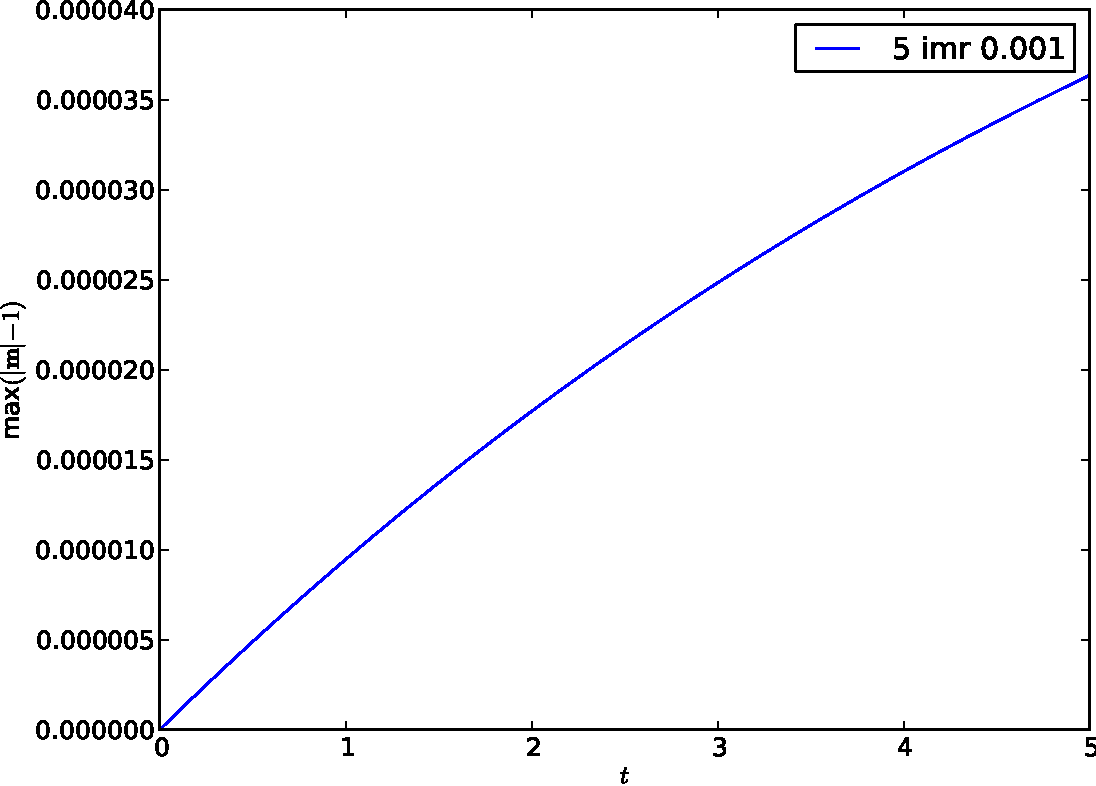
\includegraphics[width=0.8\textwidth]{plots/2d_wave_solution_m_length/gauss-maxmathbfm-1vst.pdf}
  \caption{Evolution of the maximum error of nodal magnetisation lengths in the 2D wave example with a standard Gaussian quadrature scheme.}
  \label{fig:mean-ml-error-2d-gauss}
\end{figure}

\begin{figure}
  \centering
  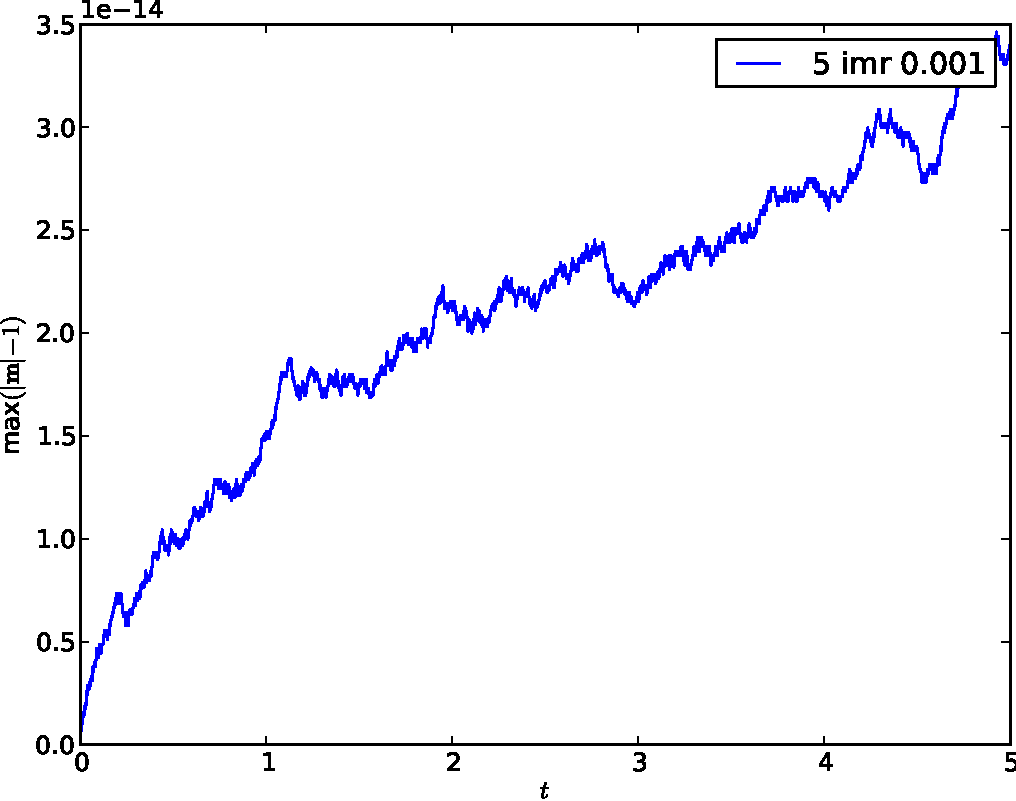
\includegraphics[width=0.8\textwidth]{plots/2d_wave_solution_m_length/lnodal-maxmathbfm-1vst.pdf}
  \caption{Evolution of the maximum error of nodal magnetisation lengths in the 2D wave example with the nodal quadrature scheme introduced above.}
  \label{fig:mean-ml-error-2d-nodal}
\end{figure}

To check that the conservation is independent of problem parameters we ran a parameter sweep using: square and triangle elements; 36, 441 and 6561 nodes; time steps of $0.1$, $0.01$ and $0.001$; and damping parameters of $1$, $0.1$, $0.001$ and $0$.
The maximum length error over all parameter sets, all time steps and all nodes when using nodal quadrature was 2.364775e-12, when using Gaussian quadrature it was 0.013746647.
This clearly demonstrates the necessity and effectiveness of the nodal quadrature scheme for retaining the conservation properties of the implicit midpoint rule.
% using the same data as for the figures above, look in their folders for parameter sets data parsing command: parse.py -d /mnt/moredata/optoomph/user_drivers/micromagnetics/experiments/parameter_sweeps/parameter_file_0/ -l=-dt -l=-damping --split=-integration --print-data max-max-ml --print-data ml -l=initial_nnode


??ds describe very long time behaviour in \cref{fig:mean-ml-error-2d-nodal-long-time}.

\begin{figure}
  \centering
  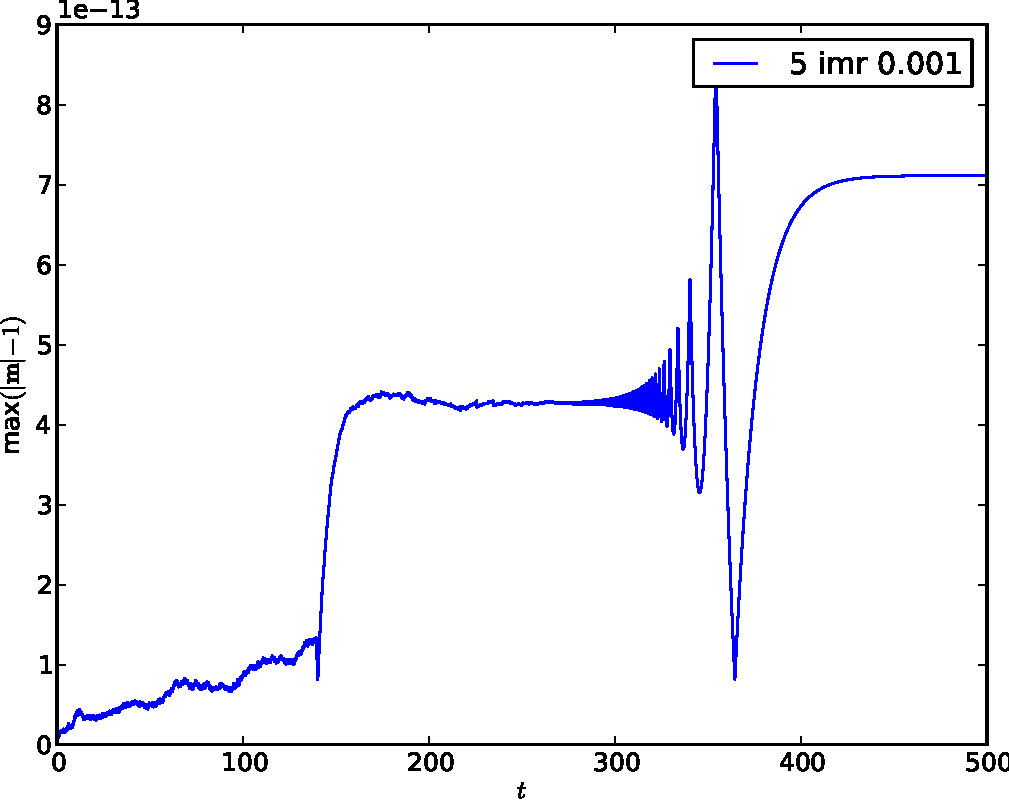
\includegraphics[width=0.8\textwidth]{plots/2d_wave_solution_m_length_long_time/-maxmathbfm-1vst.pdf}
  \caption{Evolution of the maximum error of nodal magnetisation lengths in the 2D wave example with the nodal quadrature scheme over a very long time period.}
  \label{fig:mean-ml-error-2d-nodal-long-time}
\end{figure}



\subsubsection{Effect of Newton tolerance}
\label{sec:effect-newt-toler-m-conservation}

Since the non-linear residual \cref{eq:weak-llg} used in the derivation of the conservation properties is only true up to the accuracy of the linearisation method we would expect to see some effect when modifying this accuracy.
In our model Newton's method is used for linearisation (see \cref{sec:newt-raph})so the relevant measure of accuracy is the Newton tolerance.

The obvious experiment to carry out would be to vary the Newton tolerance and examine how the error in $\abs{\mv}$ is affected.
However Newton's method extremely quickly meaning that the final residual is sometimes orders of magnitude smaller than the tolerance, this would hide any corrolation between the tolerance and the error.
Instead we plot the error against the actual maximum residual obtained (specifically: the mean over time steps of $\norm{\rv}_\infty$ after the Newton method has converged). 
The results are shown in \cref{fig:mean-ml-error-2d-nodal-newton-tests}, there is a clear corrolation between small residuals and small length errors.


\begin{figure}
  \centering
  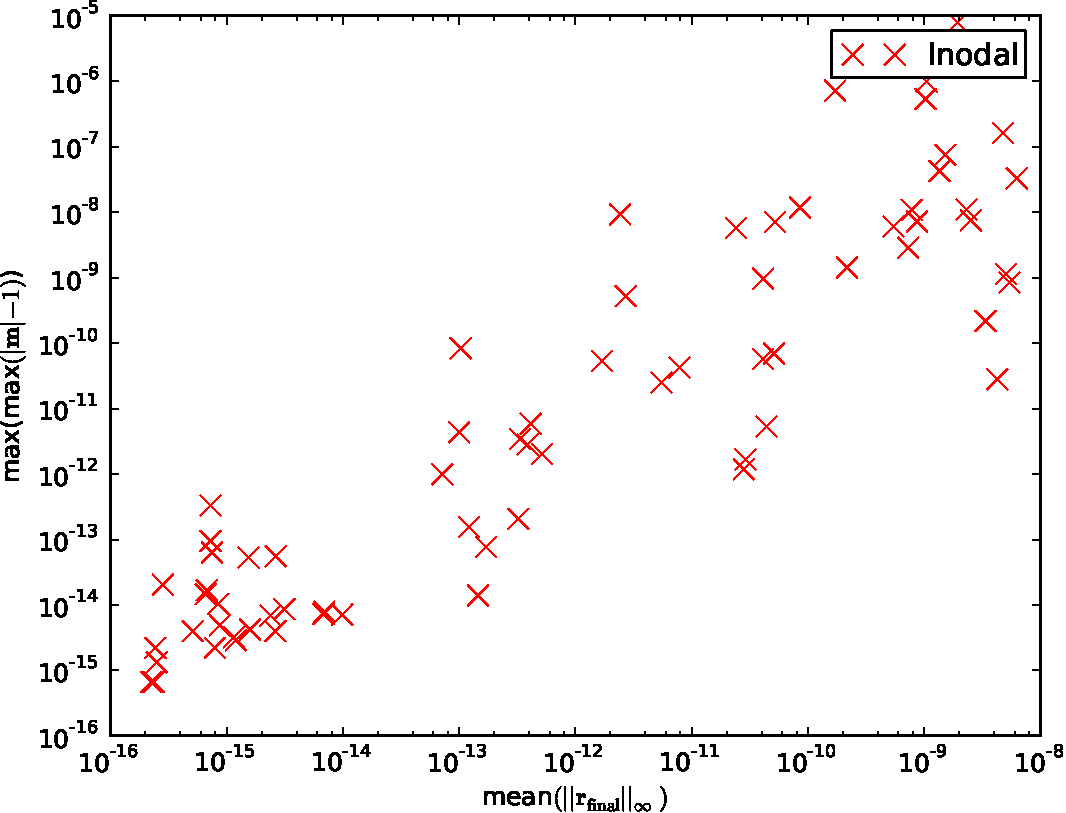
\includegraphics[width=0.8\textwidth]
  {plots/2d_wave_solution_m_length_newton_res/-maxmaxmathbfm-1vsmeanmathbfr_mathrmfinal_infty.pdf}
  \caption{Corrolation between maximum error of nodal magnetisation lengths and largest maximum Newton residual after convergence in the 2D wave example with the nodal quadrature scheme over a very long time period.}
  \label{fig:mean-ml-error-2d-nodal-newton-tests}
\end{figure}


% \subsubsection{Adaptivity}
% ??ds - no need for this? leave it to the final subsection?

% It remains to demonstrate that the adaptivity scheme introduced in \cref{sec:adaptive-imr} is effective for the finite element problem with nodal integration.
% Since there is still no relationship with previous time step sizes in the conservation proofs with nodal integration we don't expect there to be any issues with variable step size and conservation.

% Additionally our discretisation can be written as semi-discretisation in space (giving a system of ODEs) followed by the application of IMR in time.
% Hence we have no reason to expect the adaptive IMR to behave any differently to in the pure ODE case.

% \subsubsection{BEM}
% ??ds - no need for this? leave it to the final subsection?


% ??ds


\subsection{Conclusions}

??ds


%%% Local Variables:
%%% mode: latex
%%% TeX-master: "main"
%%% End:
